U ovom poglavlju predstavljeni su rezultati memorijskih i vremenskih mjerenja te su uspoređeni s prošlogodišnjom implementacijom \cite{breberic}. Mjerenja su napravljena na umjetnim i stvarnim podacima. Prilikom provedbe mjerenja diverizfikacija je postignuta različitim veličinama abecede i ulaznih sekvenci.

Sva prikazana mjerenja su dobivena na \emph{macOS High Sierra} operativnom sustavu te procesoru \emph{Intel® Core™ i7-7660U}. Sve izvršne datoteke, one naše i od kolega prošlogodišnje implementacije, su prevedene u \emph{release} konfiguraciji, što znači da je izvršni kod optimiran.

Umjetno stvoreni podaci su preuzeti od prošlogodišnjeg projekta \cite{breberic} te su sastavljeni od različitih kombinacija veličine abecede i ulaznog niza. Tako su prisutne veličine abecede $4$, $15$ i $26$ te duljine ulaznih nizova: $100, 1.000, 10.000, 100.000$ i $1.000.000$. Stvarni podaci su \emph{FASTA} datoteke preuzete s javno dostupnih baza genoma te je njihova statistika prikazana u tablici \ref{table:fasta_file_stats}.

\begin{table}[H]
  \centering
  \caption{Statistike za FASTA datoteke}
  \begin{tabular}{P{2.5cm}P{3cm}P{3cm}}
    \toprule
    Datoteka 	& Duljina niza      & Veličina abecede \\ \hline
    HIV 		& $999$	 			& $5$ \\ \hline
    E Coli 		& $5.534.367$ 		& $4$ \\ \hline
    Flu 		& $3.990$			& $4$ \\ \hline
    Camelpox 	& $205.719$ 		& $4$ \\ \hline
    Bact1 		& $1.587.120$ 		& $4$ \\
    \bottomrule
  \end{tabular}
  \label{table:fasta_file_stats}
\end{table}

\section{Memorijska mjerenja}

Tablice \ref{table:tree_mem_synt} i \ref{table:tree_mem_fasta} prikazuju zauzeće memorije stabla u dvije inačice, kodirana i nekodirana. Kodirana inačica sadrži RRR strukture koje su kodirane kako je prethodno opisano, dok nekodirana inačica ne sadrži kodirane RRR strukture, već zapisuje rang i odmak kao standardne brojeve. Tablica \ref{table:tree_mem_synt} sadrži mjerenja za umjetno stvorene nizove, dok \ref{table:tree_mem_fasta} sadrži mjerenja za stvarne nizove.

\begin{table}[H]
\centering
\caption{Potrošnja memorije stabla valića za umjetno stvorene nizove}
  \begin{tabular}{r*{6}{P{1.5cm}}}
    \toprule
    \multirow{3}{1.5cm}[-0.5em]{\centering Duljina sekvence} &  \multicolumn{6}{c}{Veličina abecede} \\
    \cmidrule(lr){2-7} 
    			& 4 & 15 & 26 & 4 & 15 & 26 \\
    \cmidrule(lr){2-7} 
    			& \multicolumn{3}{c}{Kodiran ($kB$)} & \multicolumn{3}{c}{Nekodiran ($kB$)} \\
    \hline
    100 		& $24$ & $32$ & $40$ & $24$ & $32$ & $44$ \\ \hline
    1000		& $28$ & $44$ & $56$ & $28$ & $48$ & $64$ \\ \hline
    10000		& $60$ & $140$ & $196$ & $140$ & $200$ & $264$ \\ \hline
    100000		& $420$ & $640$ & $1.088$ & $712$ & $1.400$ & $1.600$ \\ \hline
    1000000		& $3.608$ & $5.488$ & $7.152$ & $4.848$ & $8.164$ & $10.352$ \\
    \bottomrule
  \end{tabular}
  \label{table:tree_mem_synt}
\end{table}

\begin{figure}[ht]
	\centering
	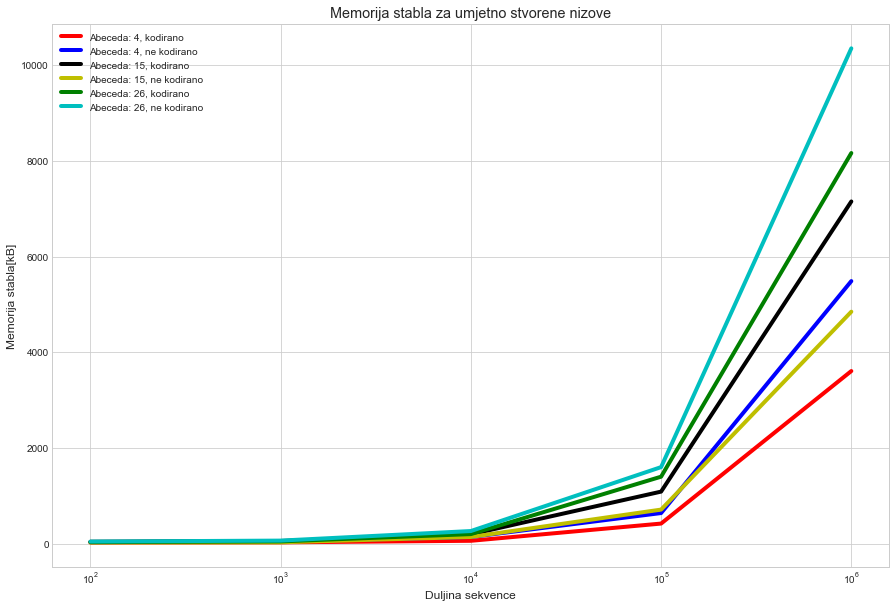
\includegraphics[width=1.0\textwidth] {graphs/graph1.png}
	\caption{Memorija stabla valića za umjetno stvorene nizove}
	\label{fig:tree_mem_synt}
\end{figure}

\begin{table}[H]
\centering
  \caption{Potrošnja memorije stabla valića za \emph{FASTA} datoteke}
  \begin{tabular}{P{2.5cm}*{2}{P{3.5cm}}}
    \toprule
    Datoteka & Kodiran ($kB$) & Nekodiran ($kB$) \\ \hline
    HIV 		& $32$ & $32$ \\ \hline
    E Coli 		& $16.240$ & $24.728$ \\ \hline
    Flu 		& $36$ & $52$ \\ \hline
    Camelpox	& $900$ & $1.008$ \\ \hline
    Bact1 		& $4.776$ & $7.312$ \\ 
    \bottomrule
  \end{tabular}
  \label{table:tree_mem_fasta}
\end{table}

Iz tablica \ref{table:tree_mem_synt} i \ref{table:tree_mem_fasta} vidljivo je da za stabla koja koriste kodiranje zauzimaju manje memorije kod većih sekvenci, od $30\%$ do $60\%$ manje memorije. Iako je zauzeće memorije manje, kodiranje uzima svoj danak prilikom izvođenja upita što je prikazano u sljedećem pod-poglavlju.

\section{Vremenska mjerenja}

Tablice \ref{table:tree_time_synt} i \ref{table:tree_time_fasta} prikazuju vrijeme potrebno za izgradnju stabla dvije inačica, kodirana i nekodirana. Tablica \ref{table:tree_time_synt} sadrži mjerenja za umjetno stvorene nizove, dok \ref{table:tree_time_fasta} sadrži mjerenja za stvarne nizove. Iz tablice \ref{table:tree_time_synt} vidljivo je kako je više vremena potrebno za izgradnju stabla sa kodiranjem za veće sekvence s većom abecedom, dok je iz tablice \ref{table:tree_time_fasta} vidljivo kako jedino za HIV potrebno više vremena za izgradnju stabla bez kodiranja, no razlika je zanemariva i vjerojatno je posljedica nepreciznosti mjerene metode.

\begin{table}[H]
\centering
\caption{Vrijeme izgradnje stabla valića za umjetno stvorene datoteke}
  \begin{tabular}{r*{6}{P{1.5cm}}}
    \toprule
    \multirow{3}{1.5cm}[-0.5em]{\centering Duljina sekvence} &  \multicolumn{6}{c}{Veličina abecede} \\
    \cmidrule(lr){2-7} 
    			& 4 & 15 & 26 & 4 & 15 & 26 \\
    \cmidrule(lr){2-7} 
    			& \multicolumn{3}{c}{Kodiran ($\mu{}s$)} & \multicolumn{3}{c}{Nekodiran ($\mu{}s$)} \\
    \hline
    100 		& $61$ & $136$ & $120$ & $61$ & $96$ & $136$ \\ \hline
    1000		& $118$ & $244$ & $280$ & $116$ & $215$ & $293$ \\ \hline
    10000		& $598$ & $1.349$ & $1.516$ & $596$ & $1.133$ & $1.478$ \\ \hline
    100000		& $5.536$ & $9.966$ & $12.819$ & $6.023$ & $14.074$ & $12.490$ \\ \hline
    1000000		& $54.351$ & $111.773$ & $133.642$ & $57.810$ & $105.501$ & $132.749$ \\
    \bottomrule
  \end{tabular}
  \label{table:tree_time_synt}
\end{table}

\begin{figure}[ht]
	\centering
	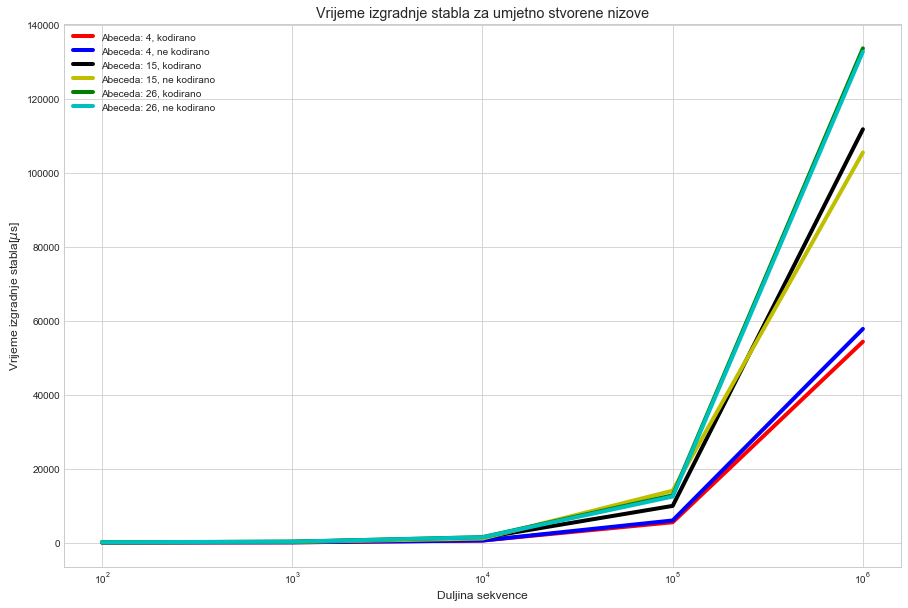
\includegraphics[width=1.0\textwidth] {graphs/graph0.png}
	\caption{Vrijeme izgradnje stabla valića za umjetno stvorene nizove}
	\label{fig:tree_time_synt}
\end{figure} 

\begin{table}[H]
\centering
  \caption{Vrijeme izgradnje stabla valića za FASTA datoteke}
  \begin{tabular}{P{2.5cm}*{2}{P{3.5cm}}}
    \toprule
    Datoteka & Kodiran ($\mu{}s$) & Nekodiran ($\mu{}s$) \\ \hline
    HIV 		& $118$           & $182$ \\ \hline
    E Coli 		& $313.131$       & $284.176$ \\ \hline
    Flu 		& $346$           & $248$ \\ \hline
    Camelpox	& $9.086$         & $8.647$ \\ \hline
    Bact1 		& $83.498$        & $77.282$ \\ 
    \bottomrule
  \end{tabular}
  \label{table:tree_time_fasta}
\end{table}

Tablice \ref{table:tree_query_time_coded_synt}, \ref{table:tree_query_time_noncoded_synt} i \ref{table:tree_query_time_fasta} prikazuju rezultate izvršavanja upita nad umjetno stvorenim i stvarnim podacima, također u dvije inačice, kodiranih i nekodiranih stabla. Isti podaci iz tablica su prikazani u obliku grafa na slikama \ref{fig:tree_rank_synt}, \ref{fig:tree_select_synt}, \ref{fig:tree_access_synt}.

\begin{table}[H]
\centering
  \caption{Prosječno vrijeme izvršavanja upita za umjetno stvorene datoteke (kodiran)}
  \begin{tabular}{r*{9}{P{1cm}}}
    \toprule
    \multirow{3}{1.3cm}[-0.5em]{\centering Duljina sekvence} &  \multicolumn{9}{c}{Veličina abecede} \\
    \cmidrule(lr){2-10} 
    			& 4 & 15 & 26 & 4 & 15 & 26 & 4 & 15 & 26 \\
    \cmidrule(lr){2-10} 
   				& \multicolumn{3}{c}{rank ($ns$)} & \multicolumn{3}{c}{select ($ns$)} & \multicolumn{3}{c}{access ($ns$)} \\
    \hline
    100 		& $229$ & $524$ & $414$    & $520$ & $1.010$ & $775$    & $509$ & $1.122$ & $805$ \\ \hline
    1000		& $248$ & $474$ & $420$    & $452$ & $860$ & $790$      & $570$ & $1.110$ & $1.025$ \\ \hline
    10000		& $369$ & $534$ & $529$    & $743$ & $1.143$ & $931$    & $855$ & $1.381$ & $1.307$ \\ \hline
    100000		& $537$ & $547$ & $665$    & $869$ & $977$ & $1.183$    & $1.176$ & $1.324$ & $1.577$ \\ \hline
    1000000		& $404$ & $898$ & $1.080$  & $679$ & $1.423$ & $1.801$  & $930$ & $1.915$ & $2.346$ \\
    \bottomrule
  \end{tabular}
  \label{table:tree_query_time_coded_synt}
\end{table}

\begin{table}[H]
\centering
  \caption{Prosječno vrijeme izvršavanja upita za umjetno stvorene datoteke (nekodiran)}
  \begin{tabular}{r*{9}{P{1cm}}}
    \toprule
    \multirow{3}{1.3cm}[-0.5em]{\centering Duljina sekvence} &  \multicolumn{9}{c}{Veličina abecede} \\
    \cmidrule(lr){2-10} 
    			& 4 & 15 & 26 & 4 & 15 & 26 & 4 & 15 & 26 \\
    \cmidrule(lr){2-10} 
   				& \multicolumn{3}{c}{rank ($ns$)} & \multicolumn{3}{c}{select ($ns$)} & \multicolumn{3}{c}{access ($ns$)} \\
    \hline
    100 		& $178$ & $274$ & $317$    & $442$ & $571$ & $693$    & $359$ & $535$ & $580$ \\ \hline
    1000		& $166$ & $243$ & $285$    & $351$ & $521$ & $605$    & $322$ & $507$ & $595$ \\ \hline
    10000		& $143$ & $249$ & $294$    & $302$ & $582$ & $663$    & $273$ & $486$ & $578$ \\ \hline
    100000		& $198$ & $337$ & $344$    & $526$ & $824$ & $856$    & $342$ & $596$ & $619$ \\ \hline
    1000000		& $217$ & $442$ & $734$    & $509$ & $926$ & $1.497$  & $365$ & $657$ & $1.037$ \\
    \bottomrule
  \end{tabular}
  \label{table:tree_query_time_noncoded_synt}
\end{table}

Iz priloženih grafova \ref{fig:tree_rank_synt}, \ref{fig:tree_select_synt}, \ref{fig:tree_access_synt}, izvršavanje upita je brže i do nekoliko puta bez kodiranja za sve veličine abeceda i sekvenci. Takav rezultat je i očekivan s obzirom da se dio vremena kod upita s kodiranjem potroši na dekodiranje.

\begin{figure}[H]
	\centering
	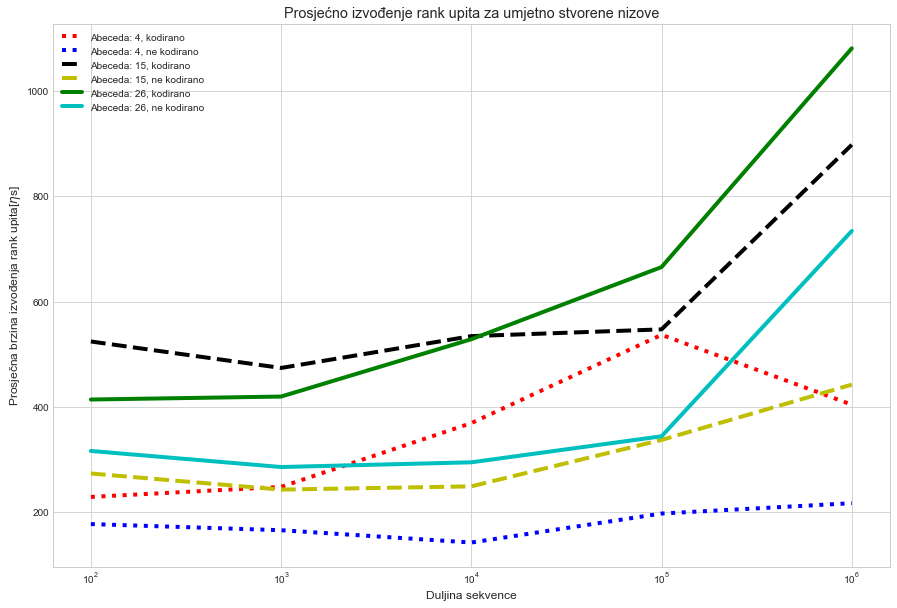
\includegraphics[width=1.0\textwidth] {graphs/graph2.png}
	\caption{Prosjećno vrijeme rank upita za umjetno stvorene nizove}
	\label{fig:tree_rank_synt}
\end{figure} 

\begin{figure}[H]
	\centering
	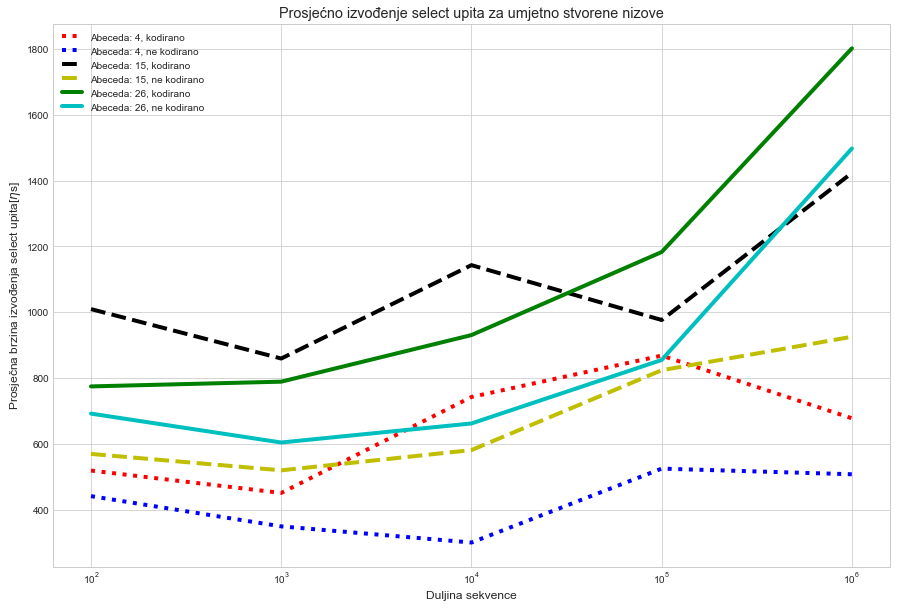
\includegraphics[width=1.0\textwidth] {graphs/graph3.png}
	\caption{Prosjećno vrijeme select upita za umjetno stvorene nizove}
	\label{fig:tree_select_synt}
\end{figure} 

\begin{figure}[H]
	\centering
	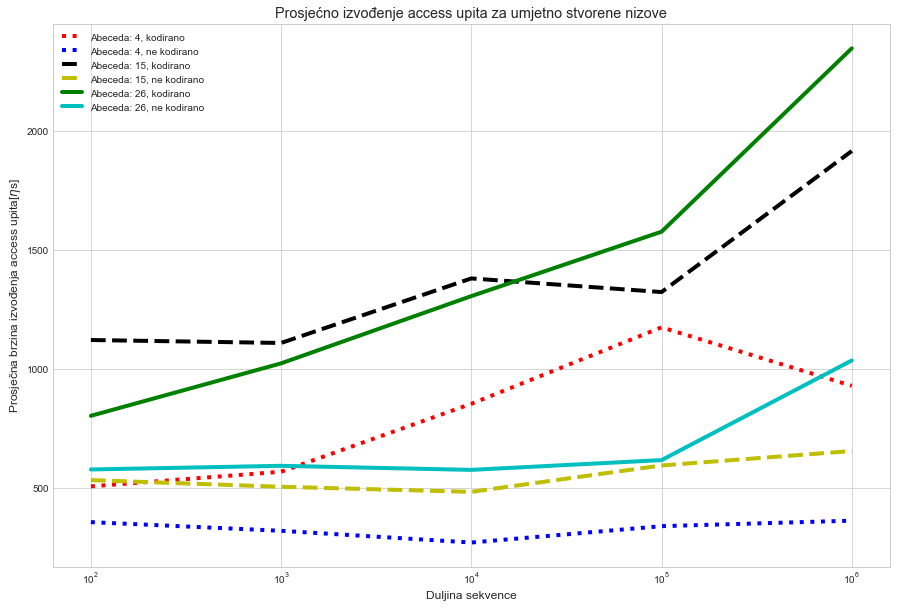
\includegraphics[width=1.0\textwidth] {graphs/graph4.png}
	\caption{Prosjećno vrijeme access upita za umjetno stvorene nizove}
	\label{fig:tree_access_synt}
\end{figure} 

\begin{table}[H]
\centering
\caption{Prosječno vrijeme izvršavanja upita za FASTA datoteke}
  \begin{tabular}{r*{6}{P{1.5cm}}}
    \toprule
    \multirow{3}{1.5cm}[-0.5em]{\centering Duljina sekvence} &  \multicolumn{6}{c}{Veličina abecede} \\
    \cmidrule(lr){2-7} & \multicolumn{3}{c}{Kodiran ($ns$)} & \multicolumn{3}{c}{Nekodiran ($ns$)} \\
    \cmidrule(lr){2-7} & rank & select & access & rank & select & access \\
    \hline
    HIV 		& $248$ & $451$ & $587$ & $251$ & $522$ & $507$ \\ \hline
    E Coli		& $473$ & $710$ & $982$ & $277$ & $532$ & $395$ \\ \hline
    Flu 		& $233$ & $412$ & $551$ & $142$ & $310$ & $279$ \\ \hline
    Camelpox	& $328$ & $605$ & $787$ & $152$ & $416$ & $277$ \\ \hline
    Bact1		& $396$ & $643$ & $893$ & $220$ & $465$ & $328$ \\
    \bottomrule
  \end{tabular}
  \label{table:tree_query_time_fasta}
\end{table}

Tablica \ref{table:tree_time_fasta} sadrži mjerenja vremena upita za stvarne nizove za implementacije s kodiranjem i bez kodiranja. Kao i na umjetno stvorenim datotekama, i na stvarnim datotekama kodiranje višestruko uspori izvođenje upita.

\section{Rezultati implementacije Brebrić, Kelemen, Volarić Horvat \cite{breberic}}

U nastavku su prikazani rezultati prošlogodišnjeg projekta \cite{breberic}.
U tablicama \ref{table:tree_mem_kel_synt} i \ref{table:tree_mem_kel_fasta} su prikazana memorijska zauzeća stabla valića. Kolege su također koristili kodiranje zapisa te su njihovi rezultati mjerenja nešto bolji, no razlog tomu leži u korištenju manje memorijske preciznosti i \emph{bug}-a u njihovom programu, te se to može uočiti na \emph{E Coli} mjerenjima u tablici \ref{table:tree_mem_kel_fasta} gdje njihov program ``podivlja'' na nizovima preko nekoliko milijuna znakova.

\begin{table}[H]
\centering
\caption{Potrošnja memorije stabla valića za umjetno stvorene datoteke}
  \begin{tabular}{r*{6}{P{1.5cm}}}
    \toprule
    \multirow{3}{1.5cm}[-0.5em]{\centering Duljina sekvence} &  \multicolumn{3}{c}{Veličina abecede} \\
    \cmidrule(lr){2-4} 
    			& 4 & 15 & 26\\
    \cmidrule(lr){2-4} 
    			& \multicolumn{3}{c}{Memorija ($kB$)} \\
    \hline
        100 & $12$ & $16$ & $20$ \\ \hline
        1000 & $16$ & $20$ & $24$ \\ \hline
        10000 & $76$ & $72$ & $80$ \\ \hline
        100000 & $396$ & $416$ & $420$ \\ \hline
        1000000 & $3.584$ & $4.848$ & $5.356$ \\
    \bottomrule
  \end{tabular}
  \label{table:tree_mem_kel_synt}
\end{table}

\begin{table}[H]
\centering
  \caption{Potrošnja memorije stabla valića za FASTA datoteke}
  \begin{tabular}{P{2.5cm}*{2}{P{3.5cm}}}
    \toprule
    Datoteka & Memorija ($kB$)\\ \hline
    HIV 		& $20$ \\ \hline
    E Coli 		& $28.136$ \\ \hline
    Flu 		& $24$ \\ \hline
    Camelpox	& $888$ \\ \hline
    Bact1 		& $4.700$ \\ 
    \bottomrule
  \end{tabular}
  \label{table:tree_mem_kel_fasta}
\end{table}


U tablicama \ref{table:tree_time_kel_synt} i \ref{table:tree_time_kel_fasta} su prikazana vremena izgradnje stabla valića. Rezultati su približno jednaki našima, no njihova izgradnja stabla je također zahvaćena već spomenutim \emph{bug}-om te problemi nastaju kod jako velikih nizova, što je vidljivo kod niza \emph{E Coli} u tablici \ref{table:tree_time_kel_fasta}.

\begin{table}[H]
\centering
\caption{Vrijeme izgradnje stabla valića za umjetno stvorene datoteke}
  \begin{tabular}{r*{6}{P{1.5cm}}}
    \toprule
    \multirow{3}{1.5cm}[-0.5em]{\centering Duljina sekvence} &  \multicolumn{3}{c}{Veličina abecede} \\
    \cmidrule(lr){2-4} 
    			& 4 & 15 & 26\\
    \cmidrule(lr){2-4} 
    			& \multicolumn{3}{c}{Vrijeme izgradnje ($\mu{}s$)} \\
    \hline
        100     & $47$      & $64$      & $87$      \\ \hline
        1000    & $95$      & $163$     & $213$     \\ \hline
        10000   & $671$     & $1.329$   & $1.779$   \\ \hline
        100000  & $5.635$   & $9.563$   & $11.834$  \\ \hline
        1000000 & $52.041$  & $106.479$ & $113.794$ \\
    \bottomrule
  \end{tabular}
  \label{table:tree_time_kel_synt}
\end{table}

\begin{table}[H]
\centering
  \caption{Vrijeme izgradnje stabla valića za FASTA datoteke}
  \begin{tabular}{P{2.5cm}*{2}{P{3.5cm}}}
    \toprule
    Datoteka & Vrijeme ($\mu{}s$) \\ \hline
    HIV 		& $98$      \\ \hline
    E Coli 		& $549.105$ \\ \hline
    Flu 		& $215$     \\ \hline
    Camelpox	& $9.801$   \\ \hline
    Bact1 		& $81.731$  \\
    \bottomrule
  \end{tabular}
  \label{table:tree_time_kel_fasta}
\end{table}

U tablicama \ref{table:tree_query_time_kel_synt} i \ref{table:tree_query_time_kel_fasta} su prikazana prosječna vremena izvršavanja upita. Rezultati su približno jednaki našima s kodiranjem, čak nešto i lošija. Kolege nisu implementirali nekodiranu inačicu stabla, stoga te rezultate nije moguće usporediti, na kako je već vidljivo i u našim rezultatima, zasigurno bi bili bolji nego u slučaju kodiranih nizova. 

\begin{table}[H]
\centering
  \caption{Prosječno vrijeme izvršavanja upita za umjetno stvorene datoteke}
  \begin{tabular}{r*{9}{P{1cm}}}
    \toprule
    \multirow{3}{1.3cm}[-0.5em]{\centering Duljina sekvence} &  \multicolumn{9}{c}{Veličina abecede} \\
    \cmidrule(lr){2-10} 
    			& 4 & 15 & 26 & 4 & 15 & 26 & 4 & 15 & 26 \\
    \cmidrule(lr){2-10} 
   				& \multicolumn{3}{c}{rank ($ns$)} & \multicolumn{3}{c}{select ($ns$)} & \multicolumn{3}{c}{access ($ns$)} \\
    \hline
    100     & $235$ & $354$ & $416$     & $297$ & $411$ & $464$     & $556$     & $808$     & $889$     \\ \hline
    1000    & $268$ & $408$ & $454$     & $318$ & $474$ & $547$     & $631$     & $982$     & $1.134$   \\ \hline
    10000   & $405$ & $610$ & $715$     & $505$ & $778$ & $893$     & $977$     & $.1543$   & $1.767$   \\ \hline
    100000  & $450$ & $634$ & $739$     & $578$ & $814$ & $964$     & $.1062$   & $1.560$   & $1.841$   \\ \hline
    1000000 & $514$ & $708$ & $1.059$   & $707$ & $974$ & $1.463$   & $.1202$   & $1.753$   & $2.536$   \\
    \bottomrule
  \end{tabular}
  \label{table:tree_query_time_kel_synt}
\end{table}

\begin{table}[H]
\centering
\caption{Prosječno vrijeme izvršavanja upita za FASTA datoteke}
  \begin{tabular}{r*{4}{P{1.5cm}}}
    \toprule
    \multirow{2}{1.5cm}[-0.5em]{\centering Duljina sekvence} 
     & \multicolumn{3}{c}{Vrijeme ($ns$)} \\
    \cmidrule(lr){2-4} & rank & select & access \\
    \hline
    HIV		 & $267$     & $325$     & $653$     \\ \hline
    E Coli	 & $1.166$   & $1.583$   & $2.806$   \\ \hline
    Flu		 & $254$     & $312$     & $614$     \\ \hline
    Camelpox & $426$     & $567$     & $1.062$   \\ \hline
    Bact1	 & $504$     & $677$     & $1.138$   \\
    \bottomrule
  \end{tabular}
  \label{table:tree_query_time_kel_fasta}
\end{table}